\documentclass[11pt]{report}
\usepackage[utf8]{inputenc}
\usepackage{mathptm}
\usepackage{newcent}
\usepackage[letterpaper]{geometry}
\usepackage{graphicx}
\usepackage[perpage]{footmisc}
\usepackage{wasysym}
\usepackage{amssymb}
\usepackage{footnote}
\usepackage{enumitem}
\def\topfraction{.99}
\def\textfraction{.01}
\def\floatpagefraction{1}
\makesavenoteenv{tabular}

\def\Ohm{$\Omega$}
\def\subfig#1#2{{\sf\small\bfseries#1}\raisebox{-.2in}{\raisebox{-.5\height}{\includegraphics[scale=.6]{#2}}}}
\def\subfigh#1#2#3{{\sf\small\bfseries#1}\raisebox{.1in}{\raisebox{-\height}{\includegraphics[height=#3]{#2}}}}
\def\sub#1{\textrm{\scriptsize#1}}


\begin{document}
\thispagestyle{empty}
\begin{centering}
  {\Huge CSchem}
  \vskip30pt

  {\large Electronic circuit layout for scientists and other part-time electrical engineers}
  \vskip60pt

  {\large Daniel A. Wagenaar}
  \vfill
  
  {Copyright (c) 2018--2022}
  
\end{centering}
\pagebreak
~
\vfill
\noindent Copyright (C) 2018--2022 Daniel A. Wagenaar\medskip

``CSchem'' is free software: you can redistribute it and/or modify
it under the terms of the GNU General Public License as published by
the Free Software Foundation, either version 3 of the License, or
(at your option) any later version.

This program is distributed in the hope that it will be useful,
but WITHOUT ANY WARRANTY; without even the implied warranty of
MERCHANTABILITY or FITNESS FOR A PARTICULAR PURPOSE.  See the
GNU General Public License for more details.

You should have received a copy of the GNU General Public License
along with this program.  If not, see http://www.gnu.org/licenses.
\pagebreak

\chapter{Introduction}

This document describes the installation and usage of ``CSchem,'' a
(hopefully) easy-to-use program for drawing electronic circuit
diagrams written by Daniel Wagenaar. A companion program, ``CPCB,''
is provided for instantiating circuits on a PCB. This program is
documented separately.

\section{Why use CSchem?}

There are any number of software packages and online options available that allow you to
draw circuit diagrams. So why should you choose CSchem? CSchem is
for you if:
\begin{itemize}
  \item You like your circuit diagrams to look ready for publication
    straight from design;
  \item You like concentrating on the principles of your circuit while
    drawing the design (and leave the specific choices of components
    until the next day);
  \item You like to have quick access to the most commonly used
    symbols;
    \item You either don't need more uncommon symbols or are willing
      to draw them in an SVG editor;
      \item You like the companion program CPCB for laying out PCBs.
\end{itemize}
%
\begin{figure}
  \mbox{}\hfill
       {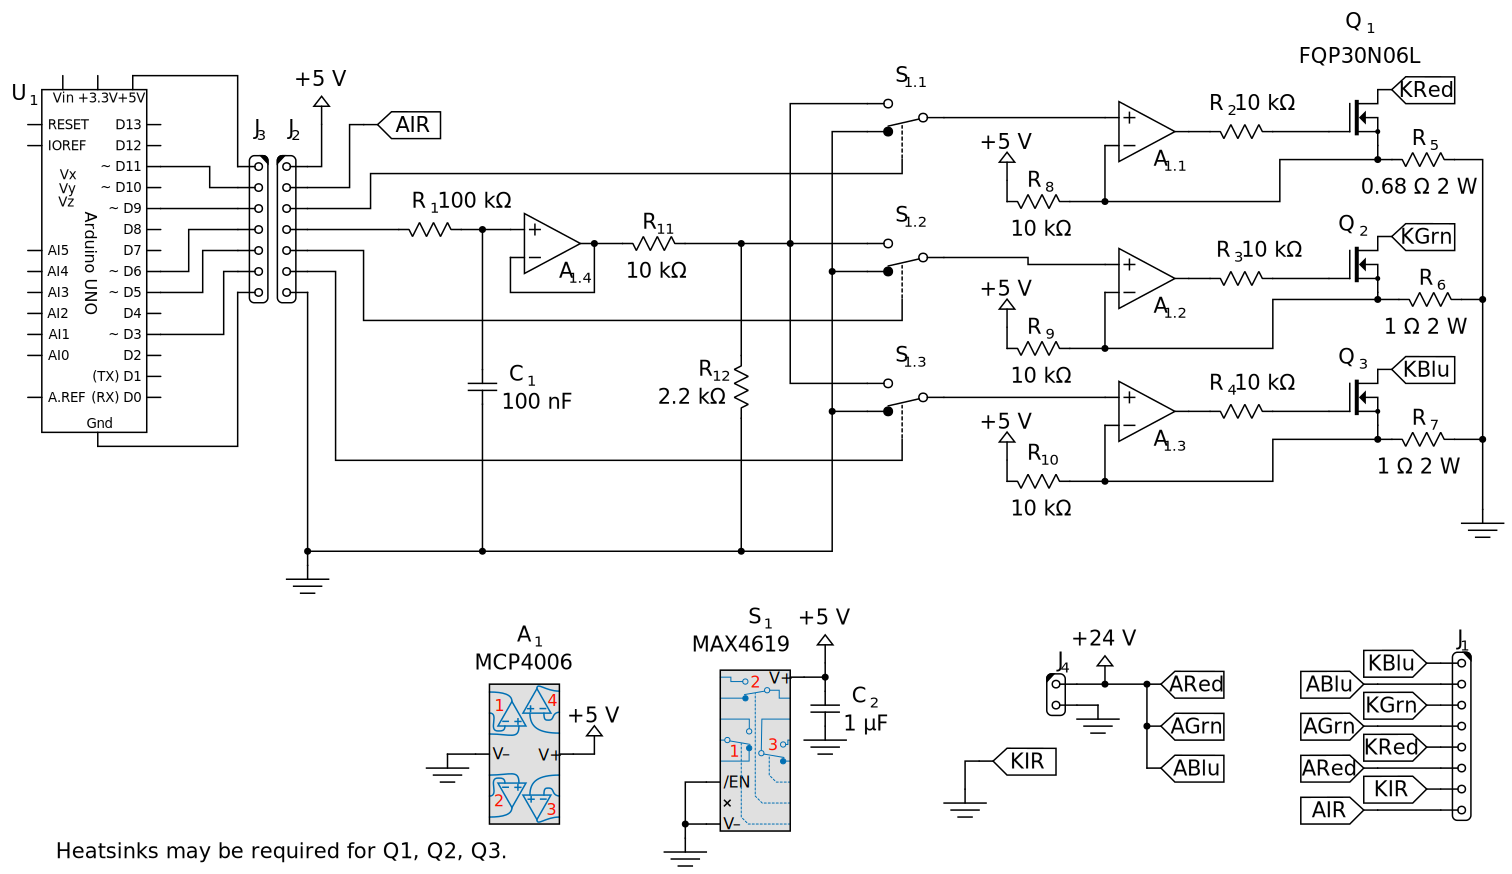
\includegraphics[width=\textwidth]{ug-driver}}
       \hfill\mbox{}
       \caption{A design
         for an Arduino-controlled triple linear LED driver as an
         example of a circuit drawn with CSchem.}
\end{figure}
%
On the other hand, CSchem may not be for you if:
\begin{itemize}
  \item You need to draw very large circuits that span multiple
    sheets;
  \item You need to specify lots of parameters with your components
    for an automated layout workflow. (CSchem will allow you to
    specify component values or part numbers, but does not have
    specific fields for vendors, packaging information, etc.)
  \item You need to have access to a large library of predrawn components.
  \item You need a help desk on call.
\end{itemize}
%
\subsection{A note on development}
CSchem is being developed by an
active research scientist. Practically, that means two things: On the
positive side, it means that I have a vested interest in fixing bugs
and improving CSchem, because I use it regularly. On the negative side, that
means that, by and large, new features are added only when I need them
and bugs are fixed when I have time. I certainly do welcome feature
requests, but I cannot guarantee that they will get implemented
quickly or at all. (If you are in a hurry, I will consider (paid)
consultancy related to CSchem.) Finally, I definitely welcome
contributions to either the code or the documentation. I would be very
happy if CSchem turned into a community-supported open source project.

\section{Features}

CSchem circuit designs consist of a single, conceptually infinitely
large sheet containing ``elements'' and ``connections.''

Elements are things like resistors and opamps, connections are simple
wires connecting between pins of elements. Each element has up to two
pieces of text associated with it: a circuit ``reference'' (e.g.,
``$R_1$,'' ``$J_2$,'' or ``$A_{3.2}$'') and a ``part/value''
designation. The ``part/value'' designation is free-form. You can use
it for a resistor value (e.g., ``10 k\Ohm'' or ``1 \Ohm{} 3 W'') or
for a part number (e.g., ``OPA2350'') or for an arbitrary
label.

Connections are wires between (pins of) elements. Where wires meet, a
``junction'' symbol is automatically inserted. Of course, wires can
also cross without electrical contact. Connections normally are
constrained to run horizontally or vertically with right-angle elbows.

The only graphical element that CSchem supports other than elements
and connections are arbitrary textual annotations that can be placed anywhere on
the sheet.

At present, CSchem does not have explicit support for buses with
multiple signal wires or for splitting a drawing across multiple sheets.

\section{Contacting the author}

If you like CSchem or find fault with it, if you discover a bug or have a
suggestion for a new feature, if you are interested in improving this
documentation or have a patch to contribute to the code, I want to
hear from you. My contact information is at
http://www.danielwagenaar.net. I very much look forward to hearing
from you. I realize that this guide is extremely terse, and I
really do welcome questions, particularly if they help me to improve
CSchem or its documentation.\bigskip

\noindent Pasadena, January 2019

\chapter{Installation}

The latest version of the software can always be downloaded from\break
http://www.danielwagenaar.net/cschem.

\section{Precompiled binaries}

Binary packages for Linux, Windows and Mac OS X will be provided as time
permits. You can help focus my attention on binaries simply by
expressing an interest.

% Installation on Windows should be easy using the provided ``CSchem.msi''
% installation package. Installation on Mac OS X should be
% straightforward by unpacking the ``CSchem-mac.tgz'' archive and placing
% ``CSchem.app'' anywhere on your hard disk.  Installation on Debian,
% Ubuntu, or Mint Linux should be equally easy using the provided
% ``CSchem.deb'' installation package. At present, installation on other
% flavors of Linux will require compiling the sources yourself, but this
% should be straightforward (see below).

% Please note that development occurs
% primarily on Linux, so the Windows and Mac OS versions may lag
% behind.

\section{Compiling the source}
To compile the source,  start from the provided
``cschem.tar.gz'' archive or check out the git source at
http://github.com/wagenadl/cschem. Compilation requires
``Qt'' version 5.6 or later.

\subsection{Compiling on Linux or Mac OS}

You will need a C++ compiler and ``make''. On Ubuntu Linux, this is as simple
as ``sudo apt-get install g++ make''. On Mac OS, you need the
``Command Line tools for XCode'' from the Apple Developers' web
site\footnote{https://developer.apple.com/xcode.}.

Open a terminal and ``cd'' to the root of the unpacked source
archive. Then type ``make'' and fetch a cup of tea. Then, either
manually copy the file ``build/cschem/cschem'' to some location on your PATH, or type ``sudo make
install'' to install into ``/usr/local/bin''.

\subsection{Compiling on Windows}

Details to follow. Again, feel free to ask!
% You will need a C++ compiler. I have successfully used both MinGW and
% Microsoft Visual Studio.
% 
% First, run ``updatesources.sh'' in the
% ``tools'' subfolder in a Cygwin shell. Then open, one by one,
% ``src/CSchem.pro''
% and ``webgrab/webgrab.pro'' in Qt
% Creator and follow the standard build steps.

\chapter{Using CSchem}

CSchem has a deliberately sparse user interface that may take a little
getting used to. It is the author's hope, however, that users will
quickly get to appreciate the simplicity of the system.

\section{Placing elements}

To place an element with a predefined symbol, simply drag the symbol
from the sidebar onto the design. To place custom elements, drag in
their SVG file from a Filer window.\footnote{E.g., Gnome Files in
  Linux, the Finder in Mac OS, or the File Explorer in Windows.} (For
more on custom elements, see section \ref{sec.custom}.) Elements can be moved around simply by dragging the mouse. To
delete an element, simply hover over it and press ``Delete.''

\section{Placing connections}

Connections can be placed starting at pins of elements simply by
dragging the mouse. The connection will start in the direction of
initial motion, so drag away from the element to avoid tangles. Click
to fixate elbows in the connection; click on a pin of an element or on
another connection to complete the connection. Press ``Return'' to
terminate a partially drawn connection and leave it dangling. Press
``Escape'' or ``Delete'' to abandon a partially drawn connection and
remove it. To start drawing a new connection starting from an existing
connection, hold ``Control'' and hover over the old connection. A
transient marker will appear just as when you hover over a pin, and
you can drag out a new connection from that point.

Existing connections can be
moved and reshaped simply by dragging the mouse. While moving,
connections will ``snap'' to nearby anchors such as pins. This
normally makes it easier to avoid spurious short zigzags. When
snapping gets in your way, simply hold ``Control'' to disable it.

Sometimes, connections and up with several unnecessary elbows. To
simplify a connection, double click on a segment that you would like
to go away. This merges the segment with the nearest segment that runs
in the same direction, eliminating also the intermediate short segment
that runs in the perpendicular direction.

To delete a connection, simply hover over it and press ``Delete.''
This only deletes the highlighted segment, but ``Control''+``B''
deletes all dangling connections, so it is easy to remove the rest.

\section{Selections and copy and paste operations}

Elements can be selected either by clicking on them or by dragging an
area around them. To add to an existing selection, hold ``Shift''
while clicking or dragging. Connections cannot be explicity selected;
instead, connections between pairs of selected elements are implicitly
selected. Use ``Control''+``C'' to copy a selection to the clipboard
or ``Control''+``X'' to cut a selection to the
clipboard. ``Control''+``V'' pastes the contents of the clipboard to
the mouse position and selects what was pasted, so that it easy to
fine position it. Normally, when dragging a selection to a new
location, junctions will be automatically inserted as needed.

\section{Adding text}

Reference and part/value labels can be added to elements that don't
already display them by double clicking on the element. These labels
will move with the element and can be micropositioned by dragging with
the mouse. To hide a label, hover over it with the mouse pointer and
press ``Backspace.'' (This doesn't actually delete the annotation; it
can be made visible again by double clicking the parent element.)

Arbitrary textual annotations can be placed anywhere on the canvas
simply by double clicking on the canvas. At present, special
formatting is not supported, but your requests will be considered. To
remove an annotation, simply delete all the text in it. (Press
``Control''+``A'' then ``Backspace'' or ``Delete.'')

\section{Exporting and printing}

CSchem does not directly talk to printers. However, it can export the
circuit diagram as vector graphics
(SVG). In addition, the parts list can be exported as a CSV file. For
further convenience, a bitmap image of the diagram can be copied to
the system clipboard for direct inclusion in, e.g., an electronic lab
notebook. Likewise, the parts list can be copied to the system clipboard.

\chapter{Advanced topics}

\section{Parts list}

To open a parts list as a side panel, use the ``View'' menu or press
``Control''+``Shift''+``L''. The parts list can be used to
conveniently modify the ``reference'' and ``part/value'' text
associated with different elements, and allows you to add arbitrary
notes to any elements. (Those notes are not displayed on the canvas.)

\section{More about elements}

It is conceptually useful to distinguish between several kinds of
elements:
\begin{description}
  \item[Ports] These are nonphysical entities such as a ground
    reference or markers to give names to signal traces.
    \item[Parts] These are mostly straightforward physical entities such as resistors,
      transistors, and connectors, but also more complex entities like
      logic gates and opamps.
    \item[Containers] These are the physical devices that contain
      one or more logic gates or opamps.
\end{description}

A few examples (Figure~\ref{parteg}) should help explain this. Ports
and simple parts are straightforward enough (Fig.~\ref{parteg}A
and~B). Virtual parts (Fig.~\ref{parteg}C) and containers
(Fig.~\ref{parteg}D) may need some explanation.

\begin{figure}[h]
  \mbox{}\hfill
  \subfig{A}{ug-ground}
  \hfill
  \subfig{B}{ug-battery}
  \hfill
  \subfig{C}{ug-opamp}
  \hfill
  \subfig{D}{ug-opamp-cont}
  \hfill\mbox{}
  \caption{Several kinds of elements. {\bf A.}~A ground reference as
    an example of a port. {\bf B.}~A battery as an example of a simple
    part. {\bf C.}~An opamp as an example of a ``virtual part.'' {\bf
      D.}~A ``container'' for two opamps.}\label{parteg}
\end{figure}


Imagine the simple amplifier circuit for a photodiode in Fig.~\ref{pdamp}.
%
\begin{figure}[h]
  \mbox{}\hfill\subfig{}{ug-pdamp}\hfill\mbox{}
  \caption{A simple photodiode amplifier.}\label{pdamp}
\end{figure}
%
In this circuit, $V_\textrm{\scriptsize out}$ is related to the photocurrent
$I_\sub{D}$ by $V_\sub{out} = R_1\;I_\sub{D}$. (To see this, consider that light
hitting a photodiode induces a photocurrent to run from the cathode to
the anode, i.e., in the reverse direction of the normal diode
current. Because the opamp $A_1$ has near-infinite input impedance,
that current can only run through $R_1$, which must therefore (Ohm's law) develop
a voltage $V = I_\sub{D}\;R_1$.) Drawing this this circuit in
this simple form is attractive for didactic purposes: including the power connections to the opamp would
make it harder to understand. However, if we are going to actually
build this circuit, we do need the opamp to be powered. Rather than
complicate the simple drawing by
drawing power connections to the opamp symbol, however, I prefer to relegate
that housekeeping stuff to a separate part of the diagram (as in Fig.~\ref{pdampcont}).
%
\begin{figure}[h]
  \mbox{}\hfill\subfig{}{ug-pdamp-cont}\hfill\mbox{}
  \caption{The photodiode amplifier with power supply
    connections.}\label{pdampcont}
\end{figure}
%
That way, the boring stuff (such as the fact that we are using a 5-V
power supply and an OPA350 opamp) does not get in the way of the
interesting stuff. Note that the virtual opamp and the container are
both labeled $A_1$, because they are ultimately one and the same when
it comes to actually building the circuit on a PCB.

\section{Drawing custom elements}\label{sec.custom}

CSchem shows the most commonly used circuit elements in a side bar. It
also ships with a folder of less commonly used elements which can be
used in a drawing simply by dragging them in from a Filer window. If
you need symbols that are not in that collection, you can draw your
own in an external SVG editor like Inkscape. The easiest way to begin
is to load one of the symbols from the supplied folder, save it under
a new name, and make edits.\footnote{I have found that starting from scratch
in a new Inkscape file tends to cause problems with scaling and
translation. This is at least partly due to a subtle bug in CSchem's handling
of SVG files which may be fixed in a future version. For now, starting
from an existing file rather than copying and pasting from an existing
file into a new file is the most practical solution.}

To make CSchem understand the structure of your file, it should
contain one single group that has all the graphics of your symbol. In
addition, the file should contain several pink circles\footnote{The color is
  not actually significant; I use pink by convention. You may not,
  however replace the circle by some other shape.} to mark pins. These
circles should not be part of the group, but exist as separate
top-level objects. Each of these circles should have a \emph{title}
tag with a specific format that identifies it as a marker for a pin
location. As an example, consider a custom symbol for a 4-diode rectifier (Fig. \ref{fig.acdc}).
%
\begin{figure}[h]
  \mbox{}\hfill
  \begin{minipage}[t]{1.5in}
    \subfig{A~}{ug-acdc}\bigskip\bigskip\\
    \subfig{C~~~~~~~~}{ug-stereo}
  \end{minipage}
  \hfill
  \subfigh{B~}{ug-acdc-screen}{1.5in}
  \hfill\mbox{}
  \caption{A custom symbol for a rectifier circuit. {\bf A.}~The
    symbol. {\bf B.}~Inkscape screenshot showing the ``title'' tag on
    one of the pin markers.} {\bf C.}~Example of a custom element
    with a placeholder for reference text.\label{fig.acdc}
\end{figure}
%
The title tag should have the form ``pin:\emph{name}'' where
\emph{name} is an arbitrary text to identify the pin. Pin names should
be chosen to reflect the function of a pin rather than the number of a
pin in any particular physical device that implements the symbol. For
instance, for a MOSFET, appropriate pin names would be ``G,'' ``D,''
and ``S'' (for Gate, Source and Drain) rather than ``1,'' ``2,'' and
``3''. If one particular numbering scheme is prevalent, it is possible
to use both numbers and a name in the title tag. For instance:
``pin:1/G'' or ``pin:3/S.''

The pink circles will not appear in CSChem; they are just to
mark the pin positions.

In addition to circles that represent pins, custom symbols may also
contain rectangles (conventionally with rounded corners) as
placeholders for annotations such as reference text
(Fig.~\ref{fig.acdc}C). These should have ``annotation:ref'' or
``annotation:value'' as their title tag.\footnote{As an alias for
  ``annotation:ref,'' ``annotation:name'' is also accepted.} If no
placeholders for annotations are included, annotations will be placed
at a default location.

Custom symbols that represent containers are slightly more complex (Fig.~\ref{fig.cont}). 
%
\begin{figure}[h]
  \mbox{}\hfill
  \subfig{A~}{ug-switchcont}
  \hfill
     \subfig{B~}{ug-switch}
     \hfill\mbox{}

   \mbox{}\hfill
   \subfig{C~~}{ug-sillyswitch}
        \hfill\mbox{}

  \caption{A custom symbol for a container for three electronic
    switches ({\bf A}) and a custom symbol for one of those switches
    ({\bf B}). Pink
    circles on the container symbol represent pins that should be wired on the
    container symbol; green circles represent pins that should be
    wired on the contents instead. {\bf C.}~A (rather silly) circuit
    demonstrating the use of these symbols.}\label{fig.cont}
\end{figure}
%
In addition to the usual pink circles, such symbols should contain
green circles to represent the pins that will be linked to the
contents of the container. These green circles must be titled
``cp:\emph{number}/\emph{index}.\emph{name},'' where \emph{number} is
the physical pin number on the standard imoplementation of the
container; \emph{index} enumerates the contained items, and
\emph{name} identifies the pin on the contained item. For example, the
switch drawn in Fig.~\ref{fig.cont}B are titled ``pin:1/nc,''
``pin:2/com,'' ``pin:3/no,'' and ``pin:4/sw.'' (For many physical
switches, pin order is ``normally closed'', ``common'', ``normally
open''; hence the numbers.) Since the container has the ``common''
terminal of the first contained switch as physical pin 4 (counting
from top-left as is conventional for a DIP IC), the green circle by
that pin is titled ``cp:4/1.com.''  CSchem automatically matches this
to the pin named ``com'' on the contained element, i.e, the circle
titled ``pin:2/com.'' (The number (``2'') is ignored for the purpose
of this matching.)  Likewise, physical pin 11 is the switch terminal
of the third contained switch, and is therefore titled ``cp:11:3/sw.''
Physical pins that have no functional connections, such as number 7 in
the example, can be titled ``cp:7/nc.'' This is not important for
CSchem, but it tells the companion program CPCB not to expect a
connection to that pin.

It is critical that the above conventions are followed
exactly. Otherwise, the symbol will not load correctly, most likely
without even an error message. (I plan to improve that situation in a
future version.)  

For visual
consistency,  the graphics of the symbol should be drawn in black
lines using the same line style (1.5-px wide, solid)
and grid spacing (7-px) as well as font (Lato). The insides of
container elements may be drawn in other colors. It may be helpful to
copy bits and pieces from several symbols to your new symbol, but
remember to create your new symbol by editing an existing file rather
than starting with an empty SVG.

\chapter{Conclusion}

I hope that CSchem will be useful to you. As mentioned before, CSchem
is in active development, and I am very interested in your thoughts
for improvement.

\end{document}
